\documentclass{article}
\usepackage[utf8]{inputenc}
%\usepackage[hidelinks]{hyperref}
\usepackage{hyperref}
\usepackage{xcolor}
\usepackage{cite}
\usepackage[version=4]{mhchem} % for isotope symbols
\usepackage{graphicx}
\usepackage[lmargin=2cm,rmargin=2cm,tmargin=2cm,bmargin=2cm,headheight=0in]{geometry}

\hypersetup{colorlinks, linkcolor={blue!50!black}, citecolor={blue!50!black},
	urlcolor={blue!50!black}}

\begin{document}
\title{Data analysis notes}
\author{Caspian Nicholls, u1027945}
\date{\today}

\maketitle

\section*{La decay data}

\medskip
\noindent
Below I outline the steps I have taken to analyse the data from experiments performed at CARIBU with the aim of exploring octupole collectivity in $\ce{^{148,150,152}Ce}$.

\begin{enumerate}
\item Work through the runbook for the afore-mentioned experiments and summarise each run.
The notes made in this step were checked by AJ Mitchell (my supervisor) who was present at the CARIBU facility when the experiments were performed and thus has a better understanding of what the notes in the run book mean.

\medskip
\noindent
This summary (located in CARIBU La decay/La\_decay\_summary.xlsx on Teams) specifically entailed noting down the run number, the beam used, the length of each run and the tape cycle that was used to collect the data.
The steps that make up each cycle are outlined below (in order).
This cycle is repeated multiple times over the course of a run.
However, the same data collection cycle was not used for all of the runs in the run book, with the \textit{beam on} and \textit{beam off} times being varied.
\begin{enumerate}
\item Record the background (typically for one second) (B/G)
\item Run the beam for some number of seconds (Beam on)
\item Record with the beam off for some number of seconds (Beam off)
\item Move the tape along to remove any sources which have long-lived activities (Tape move)
\item Record the background (again typically for one second, denoted B/G)
\end{enumerate}

\noindent
Part of this first phase is to also note whether the run was good or not, which means whether the data was recorded and nothing occurred during the run that would reduce the quality of said data.
If this quality was affected, then any indication given in the run book as to the cause was also noted down.

\medskip
\noindent
Some calibration runs were also recorded, for which the tape cycle was turned off. 

\item Check TAC (\textit{time coincidence}) spectra for coincidence data sorting so we're not missing any events by funny clock movements. 
This means checking if multiple peaks are present.
If they are, something weird has gone on with the coincidence sort codes.
\begin{enumerate}
\item Open \verb#root# (after running \verb#source ~/.profile# if it doesn't work at first).
\item \verb#.L aj-rtools.cpp# to load the macro containing tools for analysing decay data in ROOT
\item \verb#dload("filename.root")# to load in the histograms within the rootfile with name \verb#filename#. The error message \verb#fwhm.out is not found# can be safely ignored.
\item \verb#.ls# to view the histograms contained within that rootfile.
\item \verb#hist$->$ProjectionX();# generates the histogram. \verb#hist_px->Draw()# draws the histogram (which is an object called \verb#hist_px#).
\begin{figure}[htbp]
	\centering
	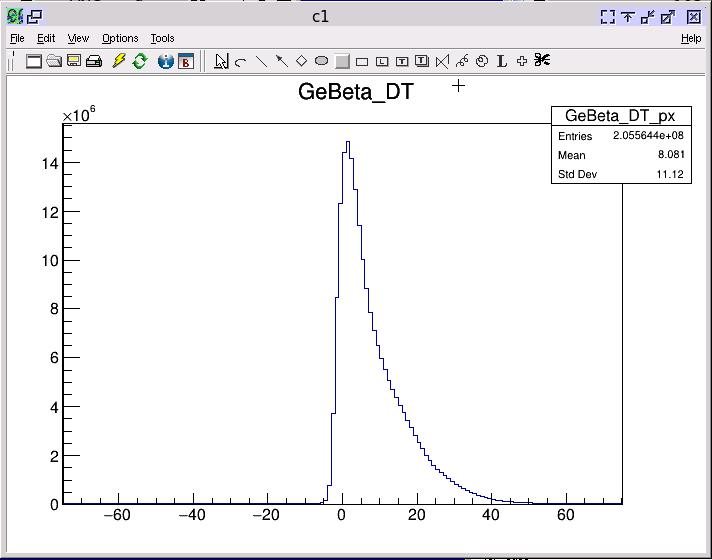
\includegraphics[width=0.5\textwidth]{../CNData/LaDecayTACspectra/148LaTACspectra.png}
	\caption{Time coincidence spectra for $\ce{^{148}La}$.}
	\label{fig:148la}
\end{figure}
\end{enumerate}
These spectra all resemble that above, with only one peak present. Thus the coincidence sort codes have worked as we would hope and no events have been missed due to `funny clock movements'.
% Note: for thesis, would want to include some vertical bars on this figure, defining the region where we make the time cuts.

\item Energy calibration. See steps in "Gain matching" note on Teams for more information. All data analysis should be performed in subdirectories of \verb#/data/# not \verb#/data10tb-ajm/# as the former is backed up every two hours, whilst the latter is backed up much less frequently. In particular, this means that if you are modifying sort codes, change them in \verb#/data/# not \verb#/data10tb-ajm/#. 
\begin{enumerate}
\item Sort with gain m=1 and offset c=0. 
For one file with run number xyz, this is achieved using the bash script \verb#gebsort_ajm.sh# (by running \verb#./gebsort_ajm.sh xyz#) and \verb#xarraycal-la.dat# with all the gain offsets set to one and zero respectively.
To sort all of the files, the bash script \verb#sortall_sh# should be used.
This just calls \verb#gebsort_ajm.sh i# for each i between 1 and however many runs were recorded.
I think that \verb#sortall_sh# may need to be modified to sort all of the files in \verb#/data10tb-ajm/caribu/ladecay/data/Merged# however, because whilst the run numbers range between 1 and 205, not all integers between 1 and 205 are included.
The calibration files don't need to be worried about however, because they are named differently to the format required by \verb#gebsort_ajm.sh#.
Looking at the `readme` in the \verb#aj_lsort# directory is also a good idea. 

\medskip
\noindent
After you have changed any sort codes, do \verb#make clean# then \verb#make ajm# to recompile them. The actual sort code is the file \verb#bin_dgs_ajm.c#, which depends on \verb#map.dat# and \verb#xarraycal-la.dat#. To sort with m = 1 and c = 0, you can either use \verb#xarraycal-zero.dat#, or modify \verb#xarraycal-la.dat# to contain only m=1 and c=0 gain parameters and use that.
\verb#xarraycal-la.dat# and \verb#xarraycal-zero.dat# are essentially just a set of parameters for each Ge crystal in the detector array.

\item Identify known room background gamma rays.
At present (in order of relative intensity) the ones used have energies (in keV) of 511, 1462, 2614, 5507, 5409 and 4218. Comparison between files in the \verb#cal# subdirectory of \verb#/data/caribu/ladecay/rootfiles# and \verb#/data10tb-ajm/caribu/ladecay/rootfiles/2020-04-14/# (or \verb#/2020-04-15/#) are used.
The former are calibrated, albeit with a dodgy calibration, but it is good enough to identify the shapes and locations of the background peaks we wish to use for the calibration.
The latter have been calibrated with m = 1 and c = 0 using \verb#gebsort\_ajm.sh#. 
\begin{enumerate}
\item This has to be done for each crystal over a suitably large range of runs (currently just starting with three; one for each distinct beam used) to achieve a good calibration. The gamma spectrum for a given crystal (e.g. crystal 5) for a given run is achieved using \verb#EhiCln->ProjectionX("px5",5,5)#.
\item The centroid channel number for the peaks of interest must be extracted using \verb#FitPanel# in ROOT. It can be done in gf3 (part of the Radware suite) but at the moment I think it is faster to do it all in ROOT.
\end{enumerate}

\item Using the average values of the centroid channel number for each peak for each crystal can then be used to identify the gain and offset parameters for each crystal, if at least two peaks are identified in each case.
More peaks will obviously give a calibration that is accurate over a wider range of energies.
The current calibration performs poorly at high energies.
This is why the data has to be recalibrated.
%%% Key point for thesis ^
Using this gain and offset then allows for a linear calibration between channel number and gamma-ray energy to be performed, by fitting the relationship between them (i.e. using a graph).

\item Update parameters in \verb#xarraycal.dat# file and resort the data with the new calibration, using \verb#sortall.sh#.

\item Add all the histograms back together (i.e. those for each channel/crystal number) and see what it looks like to check the quality of the calibration. 

\item Check the consistency of the new calibration across all the run files. Specifically, this involves checking the alignment of the energies within each run file as a function of crystal number.   
\end{enumerate}
\end{enumerate}


%\vspace*{-\baselineskip}
%\bibliographystyle{ieeetr}
%\bibliography{references.bib}{}


\end{document}